

\tikzset{every picture/.style={line width=0.75pt}} %set default line width to 0.75pt        

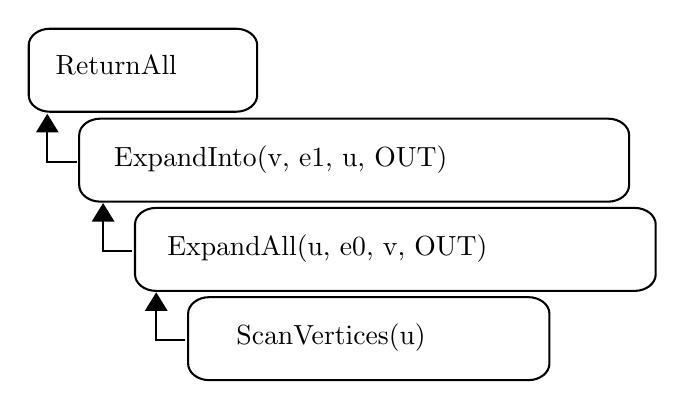
\begin{tikzpicture}[x=0.75pt,y=0.75pt,yscale=-1,xscale=1.28]
%uncomment if require: \path (0,531); %set diagram left start at 0, and has height of 531

%Rounded Rect [id:dp9370573454267987] 
\draw   (111,40) .. controls (111,35.58) and (114.58,32) .. (119,32) -- (189,32) .. controls (193.42,32) and (197,35.58) .. (197,40) -- (197,64) .. controls (197,68.42) and (193.42,72) .. (189,72) -- (119,72) .. controls (114.58,72) and (111,68.42) .. (111,64) -- cycle ;

%Rounded Rect [id:dp6856967461478435] 
\draw   (130,83.33) .. controls (130,78.91) and (133.58,75.33) .. (138,75.33) -- (329,75.33) .. controls (333.42,75.33) and (337,78.91) .. (337,83.33) -- (337,107.33) .. controls (337,111.75) and (333.42,115.33) .. (329,115.33) -- (138,115.33) .. controls (133.58,115.33) and (130,111.75) .. (130,107.33) -- cycle ;
%Straight Lines [id:da3265514824492094] 
\draw    (129,96) -- (118,96) -- (118,76) ;
\draw [shift={(118,73)}, rotate = 90] [fill={rgb, 255:red, 0; green, 0; blue, 0 }  ][line width=0.08]  [draw opacity=0] (8.93,-4.29) -- (0,0) -- (8.93,4.29) -- cycle    ;
%Rounded Rect [id:dp4438884800021361] 
\draw   (151,126.33) .. controls (151,121.91) and (154.58,118.33) .. (159,118.33) -- (339,118.33) .. controls (343.42,118.33) and (347,121.91) .. (347,126.33) -- (347,150.33) .. controls (347,154.75) and (343.42,158.33) .. (339,158.33) -- (159,158.33) .. controls (154.58,158.33) and (151,154.75) .. (151,150.33) -- cycle ;
%Straight Lines [id:da8951131696919742] 
\draw    (150,139) -- (139,139) -- (139,119) ;
\draw [shift={(139,116)}, rotate = 90] [fill={rgb, 255:red, 0; green, 0; blue, 0 }  ][line width=0.08]  [draw opacity=0] (8.93,-4.29) -- (0,0) -- (8.93,4.29) -- cycle    ;
%Rounded Rect [id:dp8868145464168437] 
\draw   (171,169.33) .. controls (171,164.91) and (174.58,161.33) .. (179,161.33) -- (299,161.33) .. controls (303.42,161.33) and (307,164.91) .. (307,169.33) -- (307,193.33) .. controls (307,197.75) and (303.42,201.33) .. (299,201.33) -- (179,201.33) .. controls (174.58,201.33) and (171,197.75) .. (171,193.33) -- cycle ;
%Straight Lines [id:da6792309496243043] 
\draw    (170,182) -- (159,182) -- (159,162) ;
\draw [shift={(159,159)}, rotate = 90] [fill={rgb, 255:red, 0; green, 0; blue, 0 }  ][line width=0.08]  [draw opacity=0] (8.93,-4.29) -- (0,0) -- (8.93,4.29) -- cycle    ;

% Text Node
\draw (120,43.5) node [anchor=north west][inner sep=0.75pt]   [align=left] {ReturnAll};
% Text Node
\draw (142,86.83) node [anchor=north west][inner sep=0.75pt]   [align=left] {ExpandInto(v, e1, u, OUT)};
% Text Node
\draw (162,129.83) node [anchor=north west][inner sep=0.75pt]   [align=left] {ExpandAll(u, e0, v, OUT)};
% Text Node
\draw (188,172.83) node [anchor=north west][inner sep=0.75pt]   [align=left] {ScanVertices(u)};


\end{tikzpicture}
